\documentclass[a4paper, 12pt, oneside]{book}
\usepackage[T1]{fontenc}
\usepackage[utf8]{inputenc}
\usepackage[portuguese]{babel}
\usepackage{graphicx}
\usepackage{float}
\graphicspath{ {./imagens/} }
\usepackage[document]{ragged2e}
\usepackage{hyphenat}
\usepackage{lipsum}

\usepackage{xcolor}
\definecolor{cinza}{rgb}{0.5,0.5,0.5}

\usepackage[a4paper]{geometry}
\geometry{left=2.5cm}
\geometry{right=2.5cm}
\geometry{footskip=2.5cm}
\setlength{\parindent}{2em}
\setlength{\parskip}{1em}
\renewcommand{\baselinestretch}{1.5}

\usepackage[sfdefault]{roboto}

\usepackage[pagestyles]{titlesec}
\newpagestyle{meuestilo}{\setfoot[\thepage][][]{\fontfamily{Montserrat-TOsF}\selectfont\color{cinza} Projectus Invictus}{}{\fontfamily{Montserrat-TOsF}\selectfont\color{cinza}\thepage}}
\pagestyle{meuestilo}

\usepackage{sectsty}
\allsectionsfont{\fontfamily{Montserrat-TOsF}\selectfont\mdseries}
\chapterfont{\raggedleft\fontfamily{Montserrat-TOsF}\selectfont\mdseries}

\usepackage{etoolbox}
\AtBeginEnvironment{quote}{\large\itshape}

\title{Título}
\author{Lucas Costa}

\begin{document}
\maketitle

\chapter*{\underline{Introdução}}

\lipsum

\noindent\makebox[\linewidth]{\rule{.5\paperwidth}{0.4pt}}

\lipsum

\chapter*{\underline{Concepção}}

\lipsum

\section*{Contato Inicial}

\lipsum


\begin{quote}
	\begin{flushright}
		\lipsum
	\end{flushright}
\end{quote}

\begin{figure}[H]
	\caption{Legenda}
	\centering
	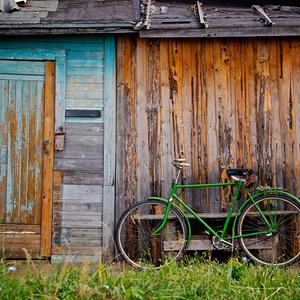
\includegraphics[width=0.8\textwidth]{76-300x300.jpg} % Figura aqui
\end{figure}

\end{document}
